\documentclass{ximera}

\input{../../../preamble.tex}


\definecolor{fvdnavy}{HTML}{071D43}
\definecolor{fvdcyan}{HTML}{20BFC6}
\definecolor{fvdcyanlight}{HTML}{EFFCFB}
\definecolor{fvdmagenta}{HTML}{F10D69}
\definecolor{fvdmagentalight}{HTML}{FFF1F7}
\definecolor{fvdtext}{HTML}{163044}





%=================================================
% Pedagogische omgevingen
% PDF: tcolorbox
% HTML: learning-box
%=================================================

\newenvironment{voorkennis}
{%
    \ifdefined\HCode
        \HCode{%
<section class="learning-box learning-box--prior">
<div class="learning-box__header">
<span class="learning-box__icon" aria-hidden="true"></span>
<span class="learning-box__title">Voorkennis</span>
</div>
<div class="learning-box__content">
        }%
        \begin{itemize}
    \else
       \begin{tcolorbox}[
    enhanced,
    breakable,
    colback=fvdcyanlight,
    colframe=fvdcyan,
    coltext=fvdtext,
    boxrule=0.5pt,
    leftrule=4pt,
    arc=4mm,
    outer arc=4mm,
    left=7mm,
    right=6mm,
    top=5mm,
    bottom=5mm,
    before skip=6mm,
    after skip=6mm,
    title=Voorkennis,
    coltitle=fvdcyan,
    fonttitle=\bfseries\Large,
    attach title to upper={\par\smallskip},
    boxed title style={
        empty,
        left=0mm,
        right=0mm,
        top=0mm,
        bottom=0mm
    },
    overlay={
        \draw[
            fvdcyan,
            line width=0.5pt
        ]
        ([xshift=42mm,yshift=-13mm]frame.north west)
        --
        ([xshift=-7mm,yshift=-13mm]frame.north east);
    }
]
        \begin{itemize}
    \fi
}
{%
    \end{itemize}
    \ifdefined\HCode
        \HCode{%
</div>
</section>
        }%
    \else
        \end{tcolorbox}
    \fi
}


\newenvironment{leerdoelen}
{%
    \ifdefined\HCode
        \HCode{%
<section class="learning-box learning-box--goals">
<div class="learning-box__header">
<span class="learning-box__icon" aria-hidden="true"></span>
<span class="learning-box__title">Leerdoelen</span>
</div>
<div class="learning-box__content">
        }%
        \begin{itemize}
    \else
\begin{tcolorbox}[
    enhanced,
    breakable,
    colback=fvdmagentalight,
    colframe=fvdmagenta,
    coltext=fvdtext,
    boxrule=0.5pt,
    leftrule=4pt,
    arc=4mm,
    outer arc=4mm,
    left=7mm,
    right=6mm,
    top=5mm,
    bottom=5mm,
    before skip=6mm,
    after skip=6mm,
    title=Leerdoelen,
    coltitle=fvdmagenta,
    fonttitle=\bfseries\Large,
    attach title to upper={\par\smallskip},
    boxed title style={
        empty,
        left=0mm,
        right=0mm,
        top=0mm,
        bottom=0mm
    },
    overlay={
        \draw[
            fvdmagenta,
            line width=0.5pt
        ]
        ([xshift=42mm,yshift=-13mm]frame.north west)
        --
        ([xshift=-7mm,yshift=-13mm]frame.north east);
    }
]
        \begin{itemize}
    \fi
}
{%
    \end{itemize}
    \ifdefined\HCode
        \HCode{%
</div>
</section>
        }%
    \else
        \end{tcolorbox}
    \fi
}


\addPrintStyle{../../..}

\title{Oefeningen --- Van kleine bijdragen naar integraal}
\author{Ingmar Herreman}

\begin{document}

% FVD_CHAPTER_DATA_START
% Automatisch gegenereerd uit index.tex.
% Niet handmatig aanpassen.
\fvdchapterdata{2}{Van oppervlakte naar integraal}{2}
% FVD_CHAPTER_DATA_END

\maketitle

\FVDbeginExercises

% ============================================================
% BASIS
% ============================================================



% ------------------------------------------------------------
% 1
% ------------------------------------------------------------

\begin{oefening}[De breedte van een deelinterval]{\oefB\ESS}

Bepaal telkens \(\Delta x\) wanneer het interval in \(n\) even brede
deelintervallen wordt verdeeld.

\begin{question}
\([0,6]\) met \(n=12\).

\begin{oplossing}
De lengte van het interval is

\[
6-0=6.
\]

Omdat we het interval in \(12\) even brede delen verdelen,

\[
\Delta x=\frac{6}{12}=\boxed{\frac12}.
\]
\end{oplossing}
\end{question}

\begin{question}
\([-2,4]\) met \(n=15\).

\begin{oplossing}
De lengte van het interval is

\[
4-(-2)=6.
\]

Dus

\[
\Delta x=\frac{6}{15}=\boxed{\frac25}.
\]
\end{oplossing}
\end{question}

\begin{question}
\([a,b]\) met \(n\) even brede deelintervallen.

\begin{oplossing}
De lengte van het interval is \(b-a\). Daarom

\[
\boxed{\Delta x=\frac{b-a}{n}}.
\]
\end{oplossing}
\end{question}

\end{oefening}


% ------------------------------------------------------------
% 2
% ------------------------------------------------------------

\begin{oefening}[Een linkersom opstellen]{\oefB\ESS}

Beschouw

\[
f(x)=x^2+2
\]

op \([0,4]\). Verdeel het interval in \(4\) even brede deelintervallen
en gebruik de linker eindpunten.

\begin{question}
Bepaal \(\Delta x\).

\begin{oplossing}
De lengte van het interval is \(4\), zodat

\[
\Delta x=\frac{4-0}{4}=\boxed{1}.
\]
\end{oplossing}
\end{question}

\begin{question}
Schrijf de linkersom op en bereken ze.

\begin{oplossing}
De deelintervallen zijn

\[
[0,1],\quad [1,2],\quad [2,3],\quad [3,4].
\]

De linker eindpunten zijn \(0,1,2,3\). We berekenen

\[
f(0)=2,\qquad
f(1)=3,\qquad
f(2)=6,\qquad
f(3)=11.
\]

Omdat \(\Delta x=1\),

\[
\begin{aligned}
L_4
&=
\left(f(0)+f(1)+f(2)+f(3)\right)\cdot1\\
&=2+3+6+11\\
&=\boxed{22}.
\end{aligned}
\]

Omdat \(f(x)=x^2+2\) stijgt op \([0,4]\), liggen deze
linkerrechthoeken onder de grafiek. De linkersom is hier dus een
onderschatting.
\end{oplossing}
\end{question}

\end{oefening}


% ------------------------------------------------------------
% 3
% ------------------------------------------------------------

\begin{oefening}[Een rechtersom opstellen]{\oefB\ESS}

Gebruik voor dezelfde functie

\[
f(x)=x^2+2
\]

op \([0,4]\) opnieuw \(4\) even brede deelintervallen, maar gebruik nu
de rechter eindpunten.

\begin{oplossing}
De rechter eindpunten zijn

\[
1,\quad2,\quad3,\quad4.
\]

We berekenen

\[
f(1)=3,\qquad
f(2)=6,\qquad
f(3)=11,\qquad
f(4)=18.
\]

Daarom

\[
\begin{aligned}
R_4
&=
\left(f(1)+f(2)+f(3)+f(4)\right)\cdot1\\
&=3+6+11+18\\
&=\boxed{38}.
\end{aligned}
\]

De functie stijgt op \([0,4]\). De rechter eindpunten geven op elk
deelinterval de grootste functiewaarde. De rechtersom is hier dus ook
de bovensom en vormt een overschatting.

Samen met de vorige oefening krijgen we

\[
\boxed{22<\text{exacte oppervlakte}<38}.
\]
\end{oplossing}

\end{oefening}


% ------------------------------------------------------------
% 4
% ------------------------------------------------------------

\begin{oefening}[Onder- en bovensom bij een dalende functie]{\oefB\ESS}

Gegeven is

\[
f(x)=9-x^2
\]

op \([0,3]\). Verdeel het interval in drie even brede deelintervallen.

\begin{center}
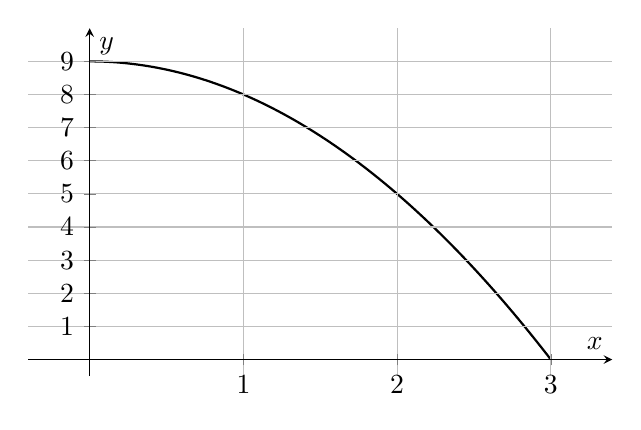
\begin{tikzpicture}
\begin{axis}[
    axis lines=middle,
    axis on top,
    xmin=-0.4, xmax=3.4,
    ymin=-0.5, ymax=10,
    xlabel={$x$},
    ylabel={$y$},
    xtick={0,1,2,3},
    ytick={0,1,2,3,4,5,6,7,8,9},
    grid=both,
    width=9cm,
    height=6cm
]
    \addplot[black,thick,domain=0:3,samples=120] {9-x^2};
\end{axis}
\end{tikzpicture}
\end{center}

\begin{question}
Bepaal \(\Delta x\).

\begin{oplossing}
Er zijn drie deelintervallen en het interval heeft lengte \(3\):

\[
\Delta x=\frac{3-0}{3}=\boxed{1}.
\]
\end{oplossing}
\end{question}

\begin{question}
Bepaal de ondersom \(s_3\) en de bovensom \(S_3\).

\begin{oplossing}
De functie \(f(x)=9-x^2\) is dalend op \([0,3]\).

Daarom ligt op elk deelinterval de kleinste functiewaarde aan het
\textbf{rechter} eindpunt. Voor de ondersom gebruiken we dus

\[
f(1)=8,\qquad f(2)=5,\qquad f(3)=0.
\]

Bijgevolg

\[
\begin{aligned}
s_3
&=f(1)\cdot1+f(2)\cdot1+f(3)\cdot1\\
&=8+5+0\\
&=\boxed{13}.
\end{aligned}
\]

Voor de bovensom gebruiken we de linker eindpunten:

\[
f(0)=9,\qquad f(1)=8,\qquad f(2)=5.
\]

Dus

\[
\begin{aligned}
S_3
&=f(0)\cdot1+f(1)\cdot1+f(2)\cdot1\\
&=9+8+5\\
&=\boxed{22}.
\end{aligned}
\]

De exacte oppervlakte \(A\) voldoet dus aan

\[
\boxed{13<A<22}.
\]
\end{oplossing}
\end{question}

\begin{question}
Welke som is hier de linkersom en welke de rechtersom?

\begin{oplossing}
Omdat de functie dalend is,

\[
\boxed{L_3=S_3=22}
\]

en

\[
\boxed{R_3=s_3=13}.
\]

Dit voorbeeld toont dat een linkersom niet automatisch een ondersom is.
\end{oplossing}
\end{question}

\end{oefening}


% ------------------------------------------------------------
% 5
% ------------------------------------------------------------

\begin{oefening}[Nog een grafische benadering]{\oefB}

Beschouw

\[
f(x)=2x^2
\]

op \([1,4]\). Verdeel het interval in drie even brede deelintervallen.

\begin{center}
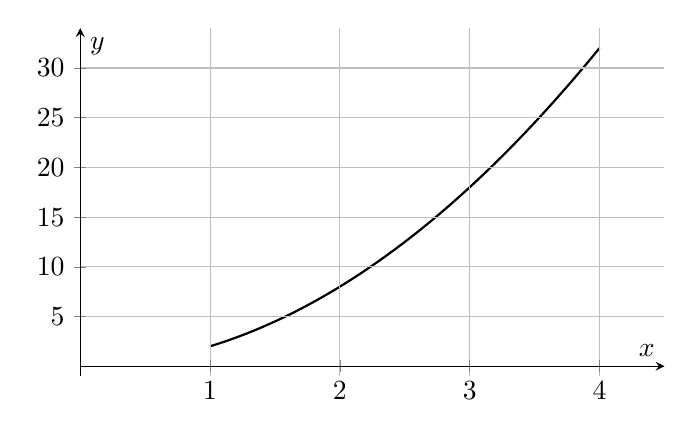
\begin{tikzpicture}
\begin{axis}[
    axis lines=middle,
    axis on top,
    xmin=0, xmax=4.5,
    ymin=-1, ymax=34,
    xlabel={$x$},
    ylabel={$y$},
    xtick={1,2,3,4},
    ytick={0,5,10,15,20,25,30},
    grid=both,
    width=9cm,
    height=6cm
]
    \addplot[black,thick,domain=1:4,samples=120] {2*x^2};
\end{axis}
\end{tikzpicture}
\end{center}

\begin{question}
Bepaal de onder- en bovensom.

\begin{oplossing}
De intervalbreedte is

\[
\Delta x=\frac{4-1}{3}=1.
\]

De functie is stijgend op \([1,4]\). De ondersom gebruikt dus de linker
eindpunten:

\[
f(1)=2,\qquad f(2)=8,\qquad f(3)=18.
\]

Daarom

\[
s_3=(2+8+18)\cdot1=\boxed{28}.
\]

De bovensom gebruikt de rechter eindpunten:

\[
f(2)=8,\qquad f(3)=18,\qquad f(4)=32.
\]

Dus

\[
S_3=(8+18+32)\cdot1=\boxed{58}.
\]

Voor de exacte oppervlakte \(A\) geldt

\[
\boxed{28<A<58}.
\]
\end{oplossing}
\end{question}

\begin{question}
Leg zonder opnieuw te rekenen uit wat je verwacht wanneer we zes in
plaats van drie even brede deelintervallen gebruiken.

\begin{oplossing}
De rechthoeken worden smaller en volgen de grafiek beter.

Omdat de functie stijgt, verwachten we dat de ondersom groter wordt en
de bovensom kleiner:

\[
s_3<s_6<A<S_6<S_3.
\]

De exacte oppervlakte wordt dus nauwer ingesloten.
\end{oplossing}
\end{question}

\end{oefening}


% ------------------------------------------------------------
% 6
% ------------------------------------------------------------

\begin{oefening}[De onderdelen van een Riemannsom]{\oefB\ESS}

Beschouw

\[
\sum_{i=1}^{10} f(x_i^\ast)\cdot0.3.
\]

\begin{question}
Welke breedte hebben de deelintervallen?

\begin{oplossing}
De factor die met de functiewaarde wordt vermenigvuldigd, is de breedte:

\[
\boxed{\Delta x=0.3}.
\]
\end{oplossing}
\end{question}

\begin{question}
Welke totale lengte heeft het interval als er \(10\) even brede
deelintervallen zijn?

\begin{oplossing}
De totale lengte is

\[
10\cdot0.3=\boxed{3}.
\]

Uit deze informatie alleen kennen we wel de lengte van het interval,
maar nog niet zijn beginpunt.
\end{oplossing}
\end{question}

\begin{question}
Wat stelt \(f(x_i^\ast)\cdot0.3\) meetkundig voor?

\begin{oplossing}
De factor \(f(x_i^\ast)\) is de gekozen hoogte en \(0.3\) is de breedte.

Daarom stelt

\[
f(x_i^\ast)\cdot0.3
\]

de georiënteerde bijdrage van één benaderingsrechthoek voor. Als
\(f(x_i^\ast)<0\), is die bijdrage negatief.
\end{oplossing}
\end{question}

\end{oefening}


% ------------------------------------------------------------
% 7
% ------------------------------------------------------------

\begin{oefening}[Lees de integraalnotatie]{\oefB\ESS}

Beschouw

\[
\int_{-2}^{5}(x^2+1)\,dx.
\]

Geef de ondergrens, bovengrens, integrand en integratievariabele.

\begin{oplossing}
We lezen rechtstreeks uit de notatie:

\[
\boxed{\text{ondergrens }=-2},
\]

\[
\boxed{\text{bovengrens }=5},
\]

\[
\boxed{\text{integrand }=x^2+1},
\]

en

\[
\boxed{\text{integratievariabele }=x}.
\]
\end{oplossing}

\end{oefening}


% ------------------------------------------------------------
% 8
% ------------------------------------------------------------

\begin{oefening}[Bereken via meetkunde]{\oefB\ESS}

Bereken zonder primitieve functies.

\begin{question}
\[
\int_0^5 4\,dx.
\]

\begin{oplossing}
De grafiek \(y=4\) vormt met de \(x\)-as op \([0,5]\) een rechthoek met
breedte \(5\) en hoogte \(4\).

Dus

\[
\int_0^5 4\,dx
=
5\cdot4
=
\boxed{20}.
\]
\end{oplossing}
\end{question}

\begin{question}
\[
\int_1^4 (-3)\,dx.
\]

\begin{oplossing}
De gewone oppervlakte van de rechthoek is

\[
(4-1)\cdot3=9.
\]

De grafiek ligt echter onder de \(x\)-as. De georiënteerde bijdrage is
dus negatief:

\[
\int_1^4(-3)\,dx=\boxed{-9}.
\]
\end{oplossing}
\end{question}

\end{oefening}


% ============================================================
% VERDIEPING
% ============================================================



% ------------------------------------------------------------
% 9
% ------------------------------------------------------------

\begin{oefening}[Linkersom, rechtersom, ondersom of bovensom?]{\oefU\ESS}

Een functie \(f\) is strikt dalend en positief op \([a,b]\). Er worden
even brede deelintervallen gebruikt.

\begin{question}
Is de linkersom een onder- of overschatting?

\begin{oplossing}
Op elk deelinterval is bij een dalende functie de functiewaarde aan het
linker eindpunt de grootste waarde.

De linkerrechthoek ligt dus boven de grafiek. Daarom is de linkersom een

\[
\boxed{\text{overschatting}}.
\]

In dit geval valt de linkersom samen met de bovensom.
\end{oplossing}
\end{question}

\begin{question}
Is de rechtersom een onder- of overschatting?

\begin{oplossing}
Aan het rechter eindpunt neemt de dalende functie op elk deelinterval
haar kleinste waarde aan.

De rechterrechthoeken liggen dus onder de grafiek. De rechtersom is een

\[
\boxed{\text{onderschatting}}.
\]

Hier valt de rechtersom samen met de ondersom.
\end{oplossing}
\end{question}

\begin{question}
Wat verandert er als \(f\) strikt stijgend is?

\begin{oplossing}
Dan is de functiewaarde aan het linker eindpunt telkens de kleinste en
aan het rechter eindpunt telkens de grootste.

Dus bij een stijgende functie:

\[
\boxed{\text{linkersom = ondersom}}
\]

en

\[
\boxed{\text{rechtersom = bovensom}}.
\]
\end{oplossing}
\end{question}

\end{oefening}


% ------------------------------------------------------------
% 10
% ------------------------------------------------------------

\begin{oefening}[Analyseer een fout]{\oefU\ESS}

Een leerling zegt:

\begin{quote}
``Een linkersom is altijd kleiner dan de bepaalde integraal.''
\end{quote}

Is dit correct? Motiveer.

\begin{oplossing}
De uitspraak is fout.

Bij een stijgende functie ligt de linkerrechthoek op elk deelinterval
onder de grafiek. De linkersom is dan een onderschatting.

Bij een dalende functie ligt de linkerrechthoek juist boven de grafiek.
De linkersom is dan een overschatting.

De keuze ``links'' of ``rechts'' bepaalt dus op zichzelf niet of een
Riemannsom groter of kleiner is dan de integraal. We moeten ook het
verloop van de functie analyseren.

\[
\boxed{\text{De uitspraak is dus niet algemeen geldig.}}
\]
\end{oplossing}

\end{oefening}


% ------------------------------------------------------------
% 11
% ------------------------------------------------------------

\begin{oefening}[Van limiet naar integraal]{\oefU\ESS}

Herken de bepaalde integraal:

\[
\lim_{n\to\infty}
\sum_{i=1}^{n}
\left(2+\left(\frac{4i}{n}\right)^2\right)
\frac{4}{n}.
\]

\begin{oplossing}
We vergelijken de uitdrukking met een Riemannsom

\[
\sum_{i=1}^n f(x_i)\Delta x.
\]

Eerst herkennen we

\[
\Delta x=\frac4n.
\]

Omdat

\[
\Delta x=\frac{b-a}{n},
\]

heeft het interval lengte \(4\). De punten

\[
x_i=\frac{4i}{n}
\]

zijn de rechter eindpunten van de verdeling van \([0,4]\).

Verder is

\[
f(x_i)=2+\left(\frac{4i}{n}\right)^2,
\]

zodat

\[
f(x)=2+x^2.
\]

Daarom

\[
\boxed{
\lim_{n\to\infty}
\sum_{i=1}^{n}
\left(2+\left(\frac{4i}{n}\right)^2\right)
\frac{4}{n}
=
\int_0^4(2+x^2)\,dx
}.
\]
\end{oplossing}

\end{oefening}


% ------------------------------------------------------------
% 12
% ------------------------------------------------------------

\begin{oefening}[Van integraal naar Riemannsom]{\oefU\ESS}

Schrijf

\[
\int_0^2(x+1)\,dx
\]

als limiet van een rechtersom met \(n\) even brede deelintervallen.

\begin{oplossing}
De intervalbreedte is

\[
\Delta x=\frac{2-0}{n}=\frac2n.
\]

Bij een rechtersom zijn de evaluatiepunten

\[
x_i=0+i\Delta x=\frac{2i}{n}.
\]

Voor \(f(x)=x+1\) krijgen we

\[
f(x_i)=1+\frac{2i}{n}.
\]

Dus

\[
\boxed{
\int_0^2(x+1)\,dx
=
\lim_{n\to\infty}
\sum_{i=1}^{n}
\left(1+\frac{2i}{n}\right)\frac2n
}.
\]
\end{oplossing}

\end{oefening}


% ------------------------------------------------------------
% 13
% ------------------------------------------------------------

\begin{oefening}[Teken en grootte van een integraal]{\oefU\ESS}

Een functie \(f\) heeft op \([0,6]\) een gebied boven de \(x\)-as met
gewone oppervlakte \(11\) en een gebied onder de \(x\)-as met gewone
oppervlakte \(15\).

\begin{question}
Bepaal

\[
\int_0^6f(x)\,dx.
\]

\begin{oplossing}
Het gebied boven de \(x\)-as levert \(+11\). Het gebied onder de
\(x\)-as levert \(-15\).

Daarom

\[
\int_0^6f(x)\,dx
=
11-15
=
\boxed{-4}.
\]
\end{oplossing}
\end{question}

\begin{question}
Bepaal de totale gewone oppervlakte tussen de grafiek en de \(x\)-as.

\begin{oplossing}
Voor de gewone oppervlakte worden beide gebieden positief geteld:

\[
11+15=\boxed{26}.
\]
\end{oplossing}
\end{question}

\begin{question}
Leg uit waarom de integraal negatief kan zijn terwijl een gewone
oppervlakte niet negatief is.

\begin{oplossing}
De bepaalde integraal stelt een \textbf{georiënteerde} oppervlakte voor.
Gebieden onder de \(x\)-as krijgen daarom een negatieve bijdrage.

Hier is de negatieve bijdrage in absolute waarde groter dan de positieve:

\[
15>11.
\]

Daarom is de netto georiënteerde bijdrage negatief.
\end{oplossing}
\end{question}

\end{oefening}


% ------------------------------------------------------------
% 14
% ------------------------------------------------------------

\begin{oefening}[Kan de integraal nul zijn?]{\oefU\ESS}

Geef een inhoudelijke verklaring waarom

\[
\int_a^b f(x)\,dx=0
\]

niet noodzakelijk betekent dat

\[
f(x)=0
\]

voor alle \(x\in[a,b]\).

\begin{oplossing}
Een integraal van nul betekent dat de totale positieve en negatieve
georiënteerde bijdragen elkaar precies opheffen.

Als bijvoorbeeld de gewone oppervlakte boven de \(x\)-as gelijk is aan
de gewone oppervlakte onder de \(x\)-as, dan

\[
S_+-S_-=0.
\]

De functie kan dus op verschillende plaatsen positief en negatief zijn,
terwijl

\[
\boxed{\int_a^b f(x)\,dx=0}.
\]

De integraal nul betekent dus niet dat de functie overal nul is.
\end{oplossing}

\end{oefening}


% ------------------------------------------------------------
% 15
% ------------------------------------------------------------

\begin{oefening}[Van steeds fijnere sommen naar een grenswaarde]{\oefU\ESS}

Voor een positieve functie \(f\) op \([0,4]\) worden de volgende
onder- en bovensommen gevonden:

\[
\begin{array}{c|c|c}
n & s_n & S_n\\
\hline
4  & 18.4 & 27.6\\
8  & 20.7 & 25.1\\
16 & 21.8 & 23.8\\
32 & 22.3 & 23.2
\end{array}
\]

\begin{question}
Wat gebeurt er met de onder- en bovensommen wanneer de verdeling fijner
wordt?

\begin{oplossing}
De ondersommen worden groter:

\[
18.4<20.7<21.8<22.3,
\]

terwijl de bovensommen kleiner worden:

\[
27.6>25.1>23.8>23.2.
\]

De twee soorten benaderingen komen dus steeds dichter bij elkaar.
\end{oplossing}
\end{question}

\begin{question}
Tussen welke waarden ligt de exacte integraal op basis van de laatste
rij?

\begin{oplossing}
De ondersom ligt onder en de bovensom boven de exacte waarde. Daarom

\[
\boxed{
22.3
<
\int_0^4f(x)\,dx
<
23.2
}.
\]
\end{oplossing}
\end{question}

\begin{question}
Leg uit hoe deze tabel het idee achter de bepaalde integraal ondersteunt.

\begin{oplossing}
Wanneer de deelintervallen smaller worden, sluiten onder- en bovensom
dezelfde waarde steeds nauwer in.

Dat ondersteunt het idee dat bij steeds fijnere verdelingen de sommen
naar één grenswaarde naderen. Die grenswaarde is precies wat we met de
bepaalde integraal beschrijven.
\end{oplossing}
\end{question}

\end{oefening}


% ============================================================
% GEVORDERD
% ============================================================



% ------------------------------------------------------------
% 16
% ------------------------------------------------------------

\begin{oefening}[Een Riemannsom reconstrueren]{\oefG}

Beschouw

\[
\lim_{n\to\infty}
\sum_{i=1}^{n}
\left(5-\frac{6i}{n}\right)^2\frac{3}{n}.
\]

Onderzoek welke bepaalde integraal deze limiet voorstelt.

\begin{oplossing}
We herkennen eerst

\[
\Delta x=\frac3n.
\]

Het interval heeft dus lengte \(3\). De punten

\[
x_i=\frac{3i}{n}
\]

zijn de rechter eindpunten van \([0,3]\).

Nu herschrijven we de functiewaarde. Omdat

\[
x_i=\frac{3i}{n},
\]

geldt

\[
\frac{6i}{n}=2x_i.
\]

Dus

\[
\left(5-\frac{6i}{n}\right)^2
=
(5-2x_i)^2.
\]

De functie is bijgevolg

\[
f(x)=(5-2x)^2.
\]

Daarom stelt de limiet de integraal

\[
\boxed{
\int_0^3(5-2x)^2\,dx
}
\]

voor.
\end{oplossing}

\end{oefening}


% ------------------------------------------------------------
% 17
% ------------------------------------------------------------

\begin{oefening}[De keuze van de evaluatiepunten]{\oefG}

Leg uit waarom de definitie van de bepaalde integraal sterker is dan de
uitspraak:

\begin{quote}
``Als de linkersommen een limiet hebben, noemen we die limiet de
integraal.''
\end{quote}

\begin{oplossing}
Een linkersom gebruikt één bijzondere keuze van evaluatiepunten:
telkens het linker eindpunt.

De bepaalde integraal moet echter een eigenschap zijn van de
\textbf{functie op het interval}, niet van één specifieke keuze van
rechthoeken.

Bij een integreerbare functie naderen de Riemannsommen bij steeds
fijnere verdelingen dezelfde grenswaarde, ook wanneer de punten
\(x_i^\ast\) binnen de deelintervallen anders gekozen worden.

Daarom is de algemene definitie met

\[
\sum_{i=1}^n f(x_i^\ast)\Delta x_i
\]

sterker dan een definitie die alleen linkersommen gebruikt.
\end{oplossing}

\end{oefening}


% ------------------------------------------------------------
% 18
% ------------------------------------------------------------

\begin{oefening}[Van benadering naar exact begrip]{\oefG}

Een leerling berekent voor een functie op \([0,2]\):

\[
L_{10}=3.72,
\qquad
R_{10}=4.18,
\]

en bij een fijnere verdeling:

\[
L_{100}=3.972,
\qquad
R_{100}=4.018.
\]

\begin{question}
Welke waarde lijkt de bepaalde integraal te hebben?

\begin{oplossing}
Zowel de linker- als de rechtersom komen bij de fijnere verdeling dicht
bij \(4\).

We verwachten daarom

\[
\boxed{
\int_0^2f(x)\,dx=4
}.
\]
\end{oplossing}
\end{question}

\begin{question}
Welke informatie ondersteunt die conclusie?

\begin{oplossing}
Bij \(n=10\) liggen de twee benaderingen nog relatief ver uit elkaar:

\[
4.18-3.72=0.46.
\]

Bij \(n=100\) is het verschil veel kleiner:

\[
4.018-3.972=0.046.
\]

Tegelijk liggen beide waarden dicht bij \(4\). De gegevens ondersteunen
dus het idee dat beide sommen bij verdere verfijning naar dezelfde
grenswaarde \(4\) naderen.
\end{oplossing}
\end{question}

\begin{question}
Kunnen we uit alleen deze vier getallen formeel bewijzen dat de integraal
exact \(4\) is?

\begin{oplossing}
Nee. De getallen geven sterke numerieke aanwijzingen, maar een eindig
aantal benaderingen vormt op zichzelf geen bewijs van de exacte
grenswaarde.

We kunnen op basis van de gegevens dus goed \textbf{vermoeden} dat de
integraal \(4\) is. Voor een exact bewijs hebben we bijkomende
wiskundige informatie nodig.
\end{oplossing}
\end{question}

\end{oefening}


\end{document}


